\documentclass[../master]{subfiles}

\begin{document}
\chapter{水蒸気混入によるドリフト速度の変化}
\label{app::drift_speed_humid_dep}
\section{水分のドリフト速度への影響}
本研究では用いた検出ガスは低圧であるため,
水分などの不純物からの影響が大きいと予想される.
そこで,チェンバー中の水分をモニターしながらドリフト速度の変化を測定した.
水分は露点計で測定した.
露点温度と水分濃度と蒸気密度の対応を表\ref{tab::dew_point_humidity}に示す.
露点温度は水が凝結を始める温度であるので,高いほどガス中に含まれる水分が多いことを示す.
測定には本文で検討した5種類の検出ガスのうち\Methane を用いた.
これは,候補とした検出ガスのうち最も圧力が低く,堆積あたりの分子数が少ないので,
不純物による影響が現れやすいと考えたためである.
この測定での各部の電圧は表\ref{tab::configuration_for_drift_dep}の通りである.
測定時は,検出ガスにを入れる前に可能な限り検出器中の水分を取るために,
半日ほど真空ポンプで排気を行った.
\begin{table}
  \centering
  \caption{露点温度と水分濃度と蒸気密度の対応.ppmはparts par millionの略であり, 10,000 ppm = \SI{1}{\percent} となる.}
  \label{tab::dew_point_humidity}
  \begin{tabular}{ccc}
    \toprule
    露点温度 (\si{\degreeCelsius}) & 水分濃度 (ppm) & 蒸気密度 (\si{\gram/\cubic\metre}) \\
    \midrule
    $-80$ & 0.540 & 0.000613 \\
    $-70$ & 2.581 & 0.00279 \\
    $-60$ & 10.67 & 0.0109 \\
    $-50$ & 38.84 & 0.0382 \\
    $-40$ & 126.7 & 0.1199 \\
    $-30$ & 375.0 & 0.339 \\
    $-20$ & 1019 & 0.884 \\
    $-10$ & 2565 & 2.14 \\
    0     & 6032 & 4.85 \\
    \bottomrule
  \end{tabular}
\end{table}
\begin{table}
  \centering
  \caption{測定で用いた電圧の構成.}
  \label{tab::configuration_for_drift_dep}
  \begin{tabular}{cc}
    \toprule
    & 電位差 (\si{\volt}) \\
    \midrule
    $\Delta V_{\text{plate-grid}}$ & 80 \\
    $\Delta V_{\text{grid-GEM}}$ & 710 \\
    $\Delta V_{\text{GEM}}$ & 410 \\
    $\Delta V_{\text{GEM-}\mu\text{-PIC}}$ & 325 \\
    $V_{\mu\text{-PIC}}$ & 175 \\
    \bottomrule
  \end{tabular}
\end{table}

時間経過によって,MAIKo チェンバー表面に吸着されていた水分が検出ガス中に放出され,検出ガスの露点温度が上昇する.
また,露点温度の上昇に伴ってドリフト速度が減少する.
露点温度とドリフト速度の時間経過を図\ref{fig::drift_time_dep}に示す.
表\ref{tab::configuration_for_drift_dep}に示したドリフト電場のとき,
Magboltz によるドリフト速度の計算値は\SI{0.0208}{\milli\metre\per\nano\second}である.
また,露点温度とドリフト速度の相関を図\ref{fig::drift_dew_dep}に示す.
\begin{figure}
  \centering
  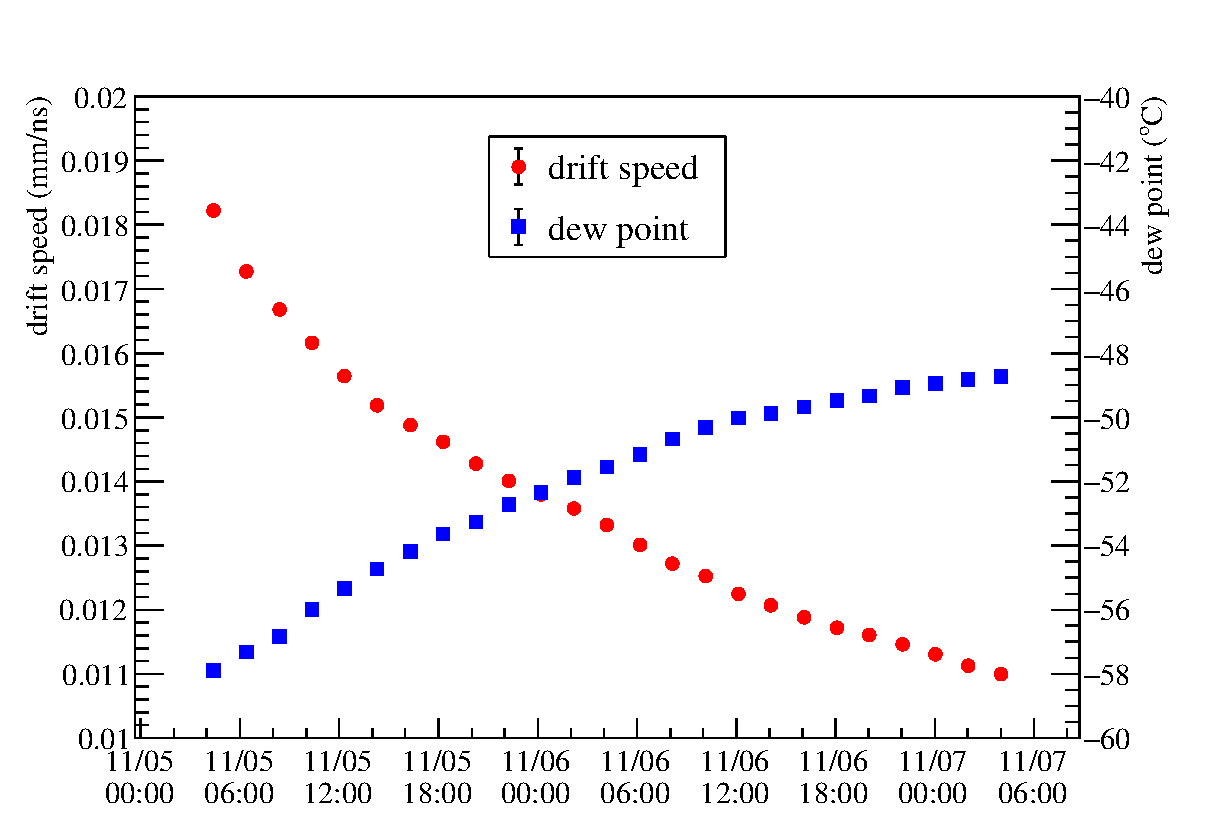
\includegraphics[clip, width=0.8\columnwidth]{drift_time_dep.eps}
  \caption[ドリフト速度と露点温度の時間変化.]
          {ドリフト速度と露点温度の時間変化.
          丸はドリフト速度,四角は露点温度,横軸は日時を表す.}
  \label{fig::drift_time_dep}
\end{figure}
\begin{figure}
  \centering
  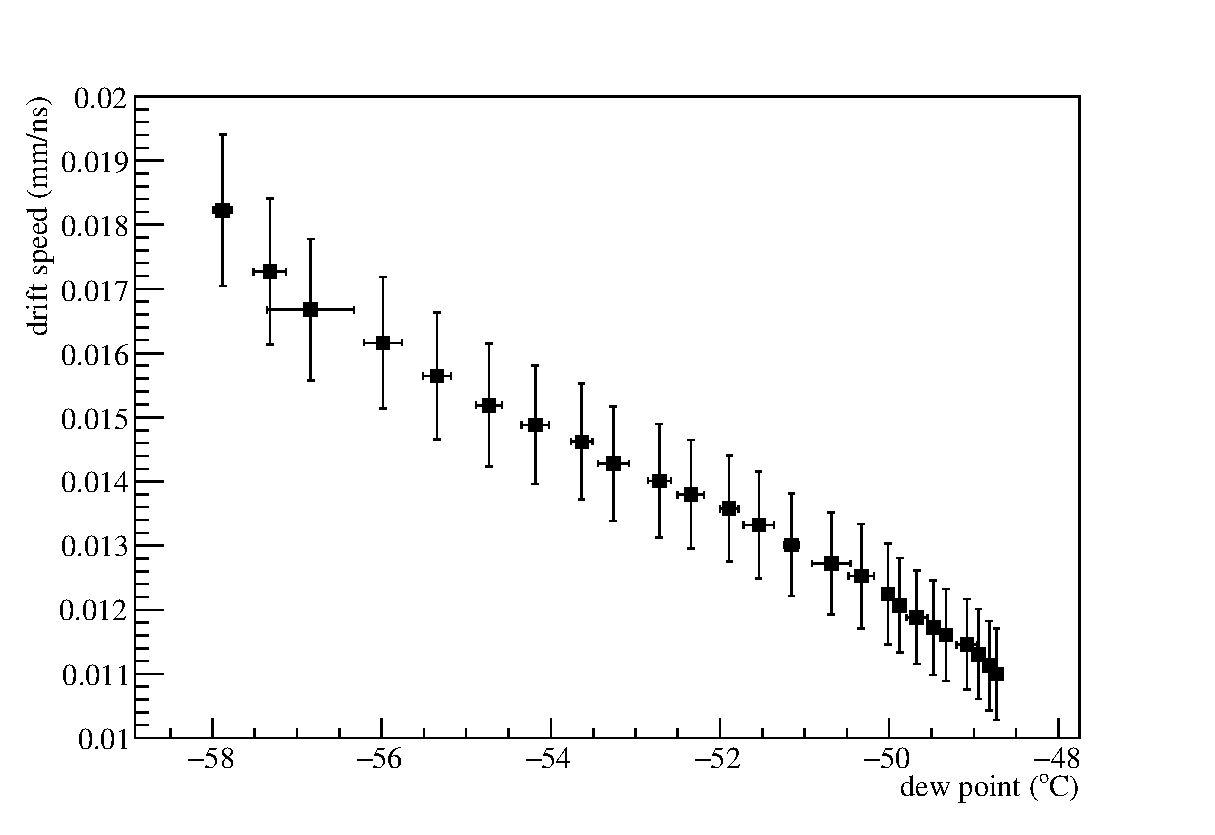
\includegraphics[clip, width=0.8\columnwidth]{drift_dew_dep.eps}
  \caption{ドリフト速度の露点温度依存性.}
  \label{fig::drift_dew_dep}
\end{figure}
%ドリフトスピードと露点温度の相関は
%\begin{equation}
%  drift\ speed =
%  -1.39
%  -7.82\times10^{-2}\times{dew\ point}
%  -1.47\times10^{-3}\times{dew\ point}^{2}
%  -9.22\times10^{-6}\times{dew\ point}^{3}
%\end{equation}
%と表すことができる.
%\begin{figure}
%  \centering
%  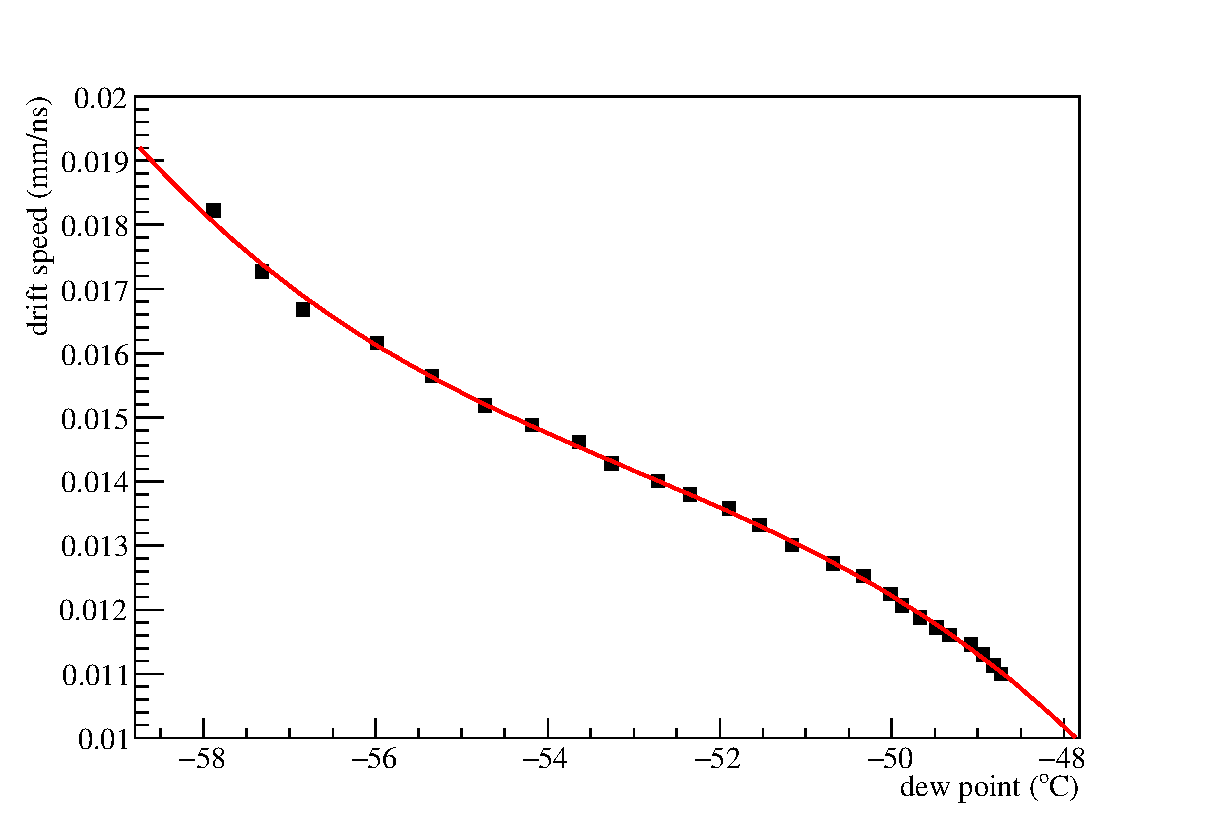
\includegraphics[clip, width=0.8\columnwidth]{drift_dew_dep_fit.eps}
%  \caption{ドリフトスピードの露点温度依存性.}
%  \label{fig::drift_dew_dep_fit}
%\end{figure}

\section{ガスフローによるガス中の水分の変化}
前節で述べたように時間経過とともにチェンバー表面から水分が放出される.
検出ガスをフローさせることで,この影響の低減を試みた.
図\ref{fig::gas_duct}に示すように,MAIKo チェンバーのinlet からガスを注入し,
outlet からポンプで排気することで,
ガスが長時間チェンバー中に留まらないようにした.
図\ref{fig::gas_duct}中の ``MFC'', ``PV'', ``MV'', ``FM'', ``SP'' はそれぞれ,
マスフローコントローラ,ピエゾバルブ,メータリングバルブ,フローメータ,スクロールポンプを表す.
ピエゾバルブとメータリングバルブで検出ガスの流量を調整するくことで,
チェンバー内の圧力を一定に保ったまま検出ガスを循環させた.
図\ref{fig::drift_time_cont}にドリフト速度と露点温度の時間経過を示す.
点線より左側では検出ガスを循環させて,右側では循環させずに測定した.
検出ガスを循環させると露点温度,ドリフト速度ともに変化が小さいことが分かる.
\begin{figure}
  \centering
  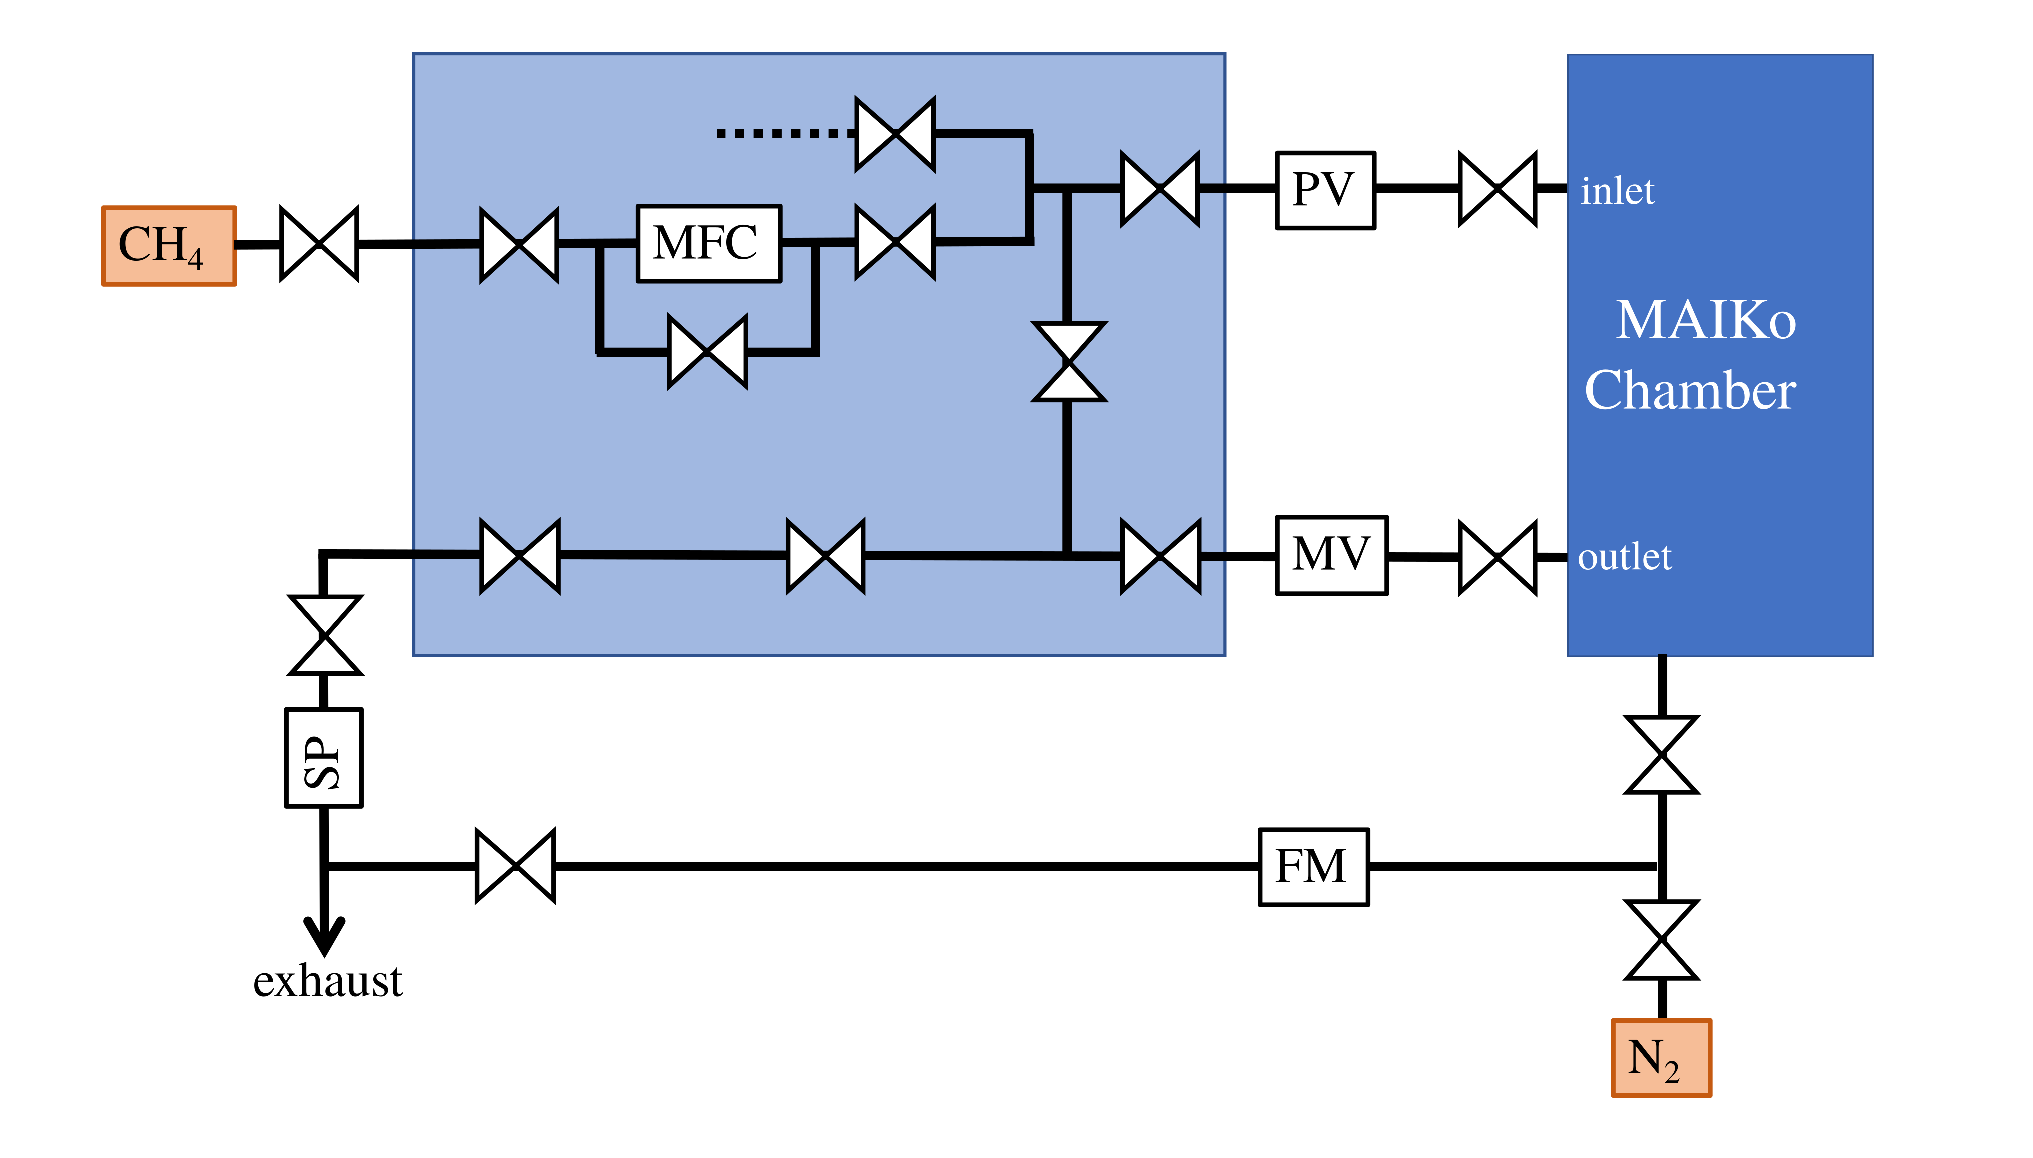
\includegraphics[clip, width=\columnwidth]{FlowDuct_ver2.eps}
  \caption{ガス配管の概観図.}
  \label{fig::gas_duct}
\end{figure}
\begin{figure}
  \centering
  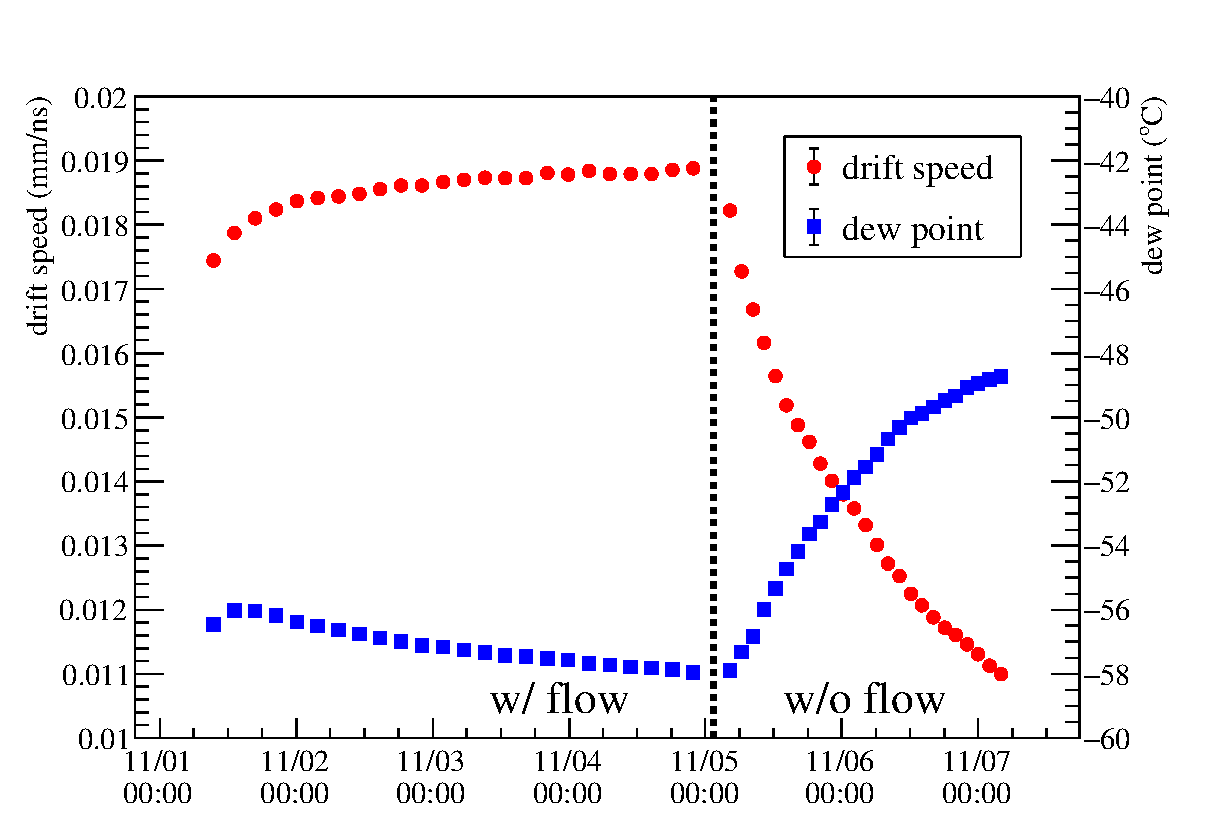
\includegraphics[clip, width=0.8\columnwidth]{drift_time_cont.eps}
  \caption{ドリフト速度と露点温度の時間経過.
  丸はドリフト速度,四角は露点温度を表す.}
  \label{fig::drift_time_cont}
\end{figure}

連続した測定で検出ガスの循環の有無で露点温度とドリフト速度の変化の違いが分かった.
このことより,チェンバー表面から多くの水分が検出ガスに放出されていることが確認された.
また,ドリフトスピードがMagboltz の計算値より小さくなる主な原因が検出ガス中に含まれる水分であることが分かった.
この影響を抑える方法として,今回行ったガスを循環させる方法が有効である.
他の方法として,チェンバー中の水分を長時間に渡ってポンプで排気することで,
チェンバー表面の水分量を減らすことも有効であると考えられる.
さらに,この2つの方法のどちらも行うことで,低い露点温度で安定して測定を行うことができると考える.

\end{document}
